\chapter{Results and Discussion}

\section{Performance analysis}

\subsection{Key metrics}

There are three key metrics that will be used to assess system performance impacts: the HTTP response time, throughput and the error rate. Within the context of self-adaptive systems, as described by \citeauthor{weyns_engineering_2018} \cite{weyns_engineering_2018}, there are two levels of a system that can be optimised. Improvements can be made to the inner managed system, or to the outer managing system. For the Ahuora Digital Platform, the optimisation explored here will focus on optimisation of the managing system, or the Kubernetes cluster. These metrics will serve to inform steps towards such optimisation.

\subsubsection{Response time}

The response time for an individual request is the total length of time taken to receive a response from a destination endpoint. This includes the duration of all steps involved in the request, including the time taken to establish an initial connection, perform a TLS handshake, wait for the response, and receive the data. As a metric, it allows an analyst to observe how a system responds over time to increasing load, with a worsening response time indicating that the system is being throttled or is reaching a performance ceiling. From a developer perspective, the response time is important to track, as an increasing response time worsens the experience for users of a product, who may perceive a slowly responding application as a reflection of poor software quality.

Response times will be assessed using an exponentially-weighted moving average (EWMA), along with comparisons at different moving percentiles. Use of a rolling median would appear either too unstable with a small window, or lag behind in showing recent trends. Using an EWMA allows recent data to be paid more attention, and enables better correlation analysis to be conducted.

\subsubsection{Throughput}

The throughput of a system is the number of requests that are processed per second. This metric can be used to identify the peak capacity of the system, as well as identify the thresholds or points at which system performance degrades. As opposed to the response time, which is concerned with the performance of individual requests, throughput is a metric that provides insight only with respect to behaviour of the overall system. One goal within a performance optimisation context is to maximise the peak throughput of a system to serve more users concurrently.

\subsubsection{Error rate}

Along with speed-oriented metrics like the response time and throughput, it is critical to keep track of the error rate, or the proportion of HTTP requests that failed. Error rates can increase under overloaded system conditions, and can provide early indication that a sustainable throughput threshold has been passed. Another reason to record errors is to ensure that they do not cause invalid observations to be made about test data. In some situations, failed requests may have lower response times than their successful counterparts, which may mislead one to think the system is more responsive than it actually is.

\subsection{Secondary metrics}

\subsubsection{Container-level resource utilisation}

Both CPU and memory usage will provide additional insight into system performance influences. For example, the observation of high consumption of allocated CPU time within a pod or container at the same time as observed request rate instability would possibly indicate the pod is reaching computation limits.

\subsubsection{Cluster-level resource allocation and utilisation}

Especially when auto-scaling policies are in place, it is necessary to track the number of deployed pods for each active cluster deployment. This metric can then be used to calculate the sum of all provisioned resources on the cluster, such as the total requested CPU. With this information, the level of over or under-provisioning can be compared across different workloads, and across workload configuration variations. If a pod requests 2000 millicores of CPU, but only uses 100 millicores on average, then this is a clear sign of severe over-provisioning. Likewise, requesting 500 millicores but quickly reaching an average of 90\% CPU utilisation would indicate under-provisioning. With auto-scaling policies in place, poorly set CPU or memory requests can rapidly multiply into cluster-wide resource allocation issues, such as additional pods being unschedulable.

\subsection{Summary statistics}

Using the data generated within tests, a number of summary statistics for each test result can be derived to assist with immediate comparison of deployment configurations.

\begin{itemize}[itemsep=0pt]
    \item \textbf{Average (mean) request completion rate}: The mean number of requests that were successfully completed per second.
    \item \textbf{Maximum request completion rate}: The peak request completion rate across the test duration.
    \item \textbf{Maximum request start rate}: The peak number of requests started by the k6 test client per second.
    \item \textbf{Average (median) response time}: The median time taken for a request to receive a response.
    \item \textbf{Overall error rate}: The proportion of requests across the test that failed due to an HTTP error or client timeout.
    \item \textbf{Performance degradation threshold}: The point at which the response time exceeds a certain level (100 milliseconds for UOR tests, and 1000 milliseconds for FS tests). This statistic allows for an approximation of the request start and completion rates where system performance begins to degrade rapidly. This threshold will not be calculated for average load or stress load tests.
    \item \textbf{Maximum started and completed request ratio}: The largest ratio between the number of requests that have started and the number that have completed. A high ratio indicates that the system is failing to process as many requests as it is receiving. This will not be calculated for breakpoint load tests.
    \item \textbf{Maximum cluster CPU request proportion}: The peak proportion of available cluster CPU used by a deployment. This will be calculated for the Django and IDAES pods only, and only for the resource allocation and utilisation tests.
\end{itemize}

\subsection{Rolling window statistics}

\section{Unit operation retrieval (UOR) experiment results}

\subsection{Benchmarks}

\begin{figure}[H]
    
    \centering
    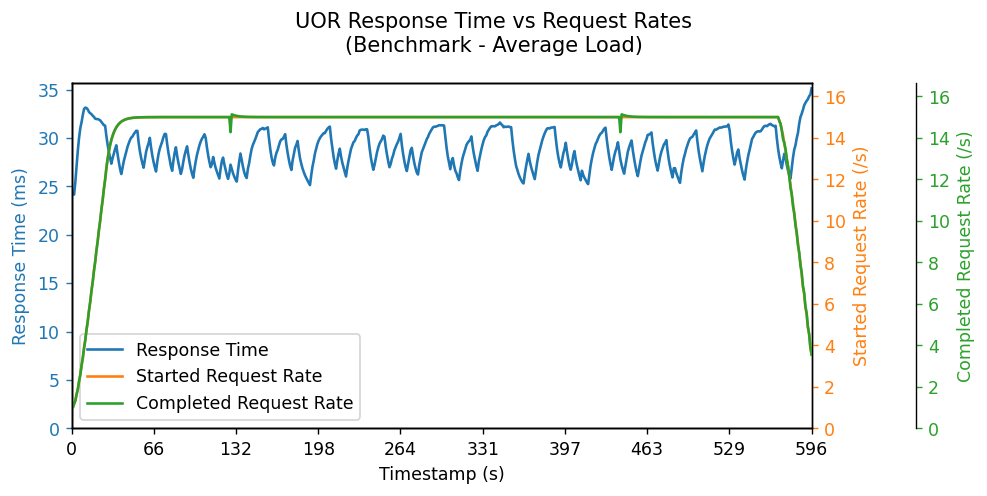
\includegraphics[width=0.8\textwidth]{figures/uor-benchmark-average.png}
    \caption{UOR response time vs. request rate graph - average load benchmark}
    \label{figure:uor-benchmark-average}
\end{figure}

\begin{figure}[H]
    \centering
    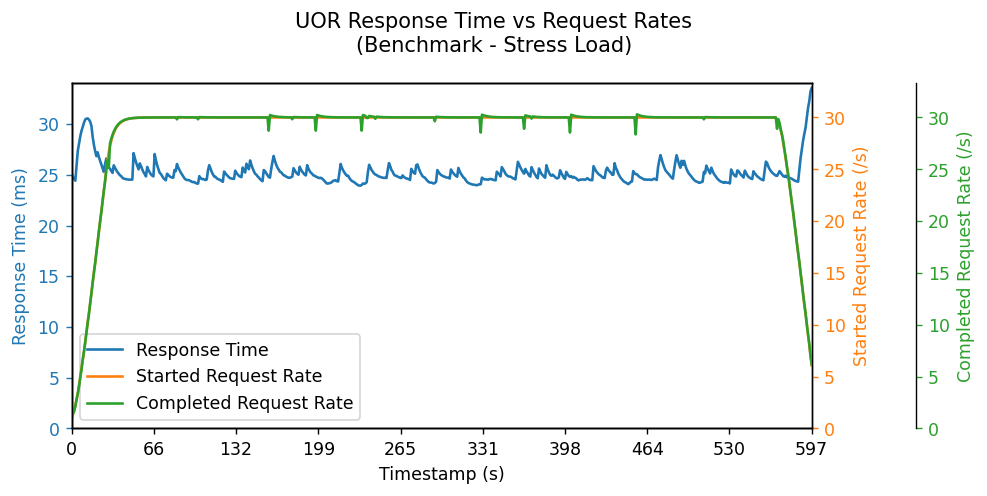
\includegraphics[width=0.8\textwidth]{figures/uor-benchmark-stress.png}
    \caption{UOR response time vs. request rate graph - stress load benchmark}
    \label{figure:uor-benchmark-stress}
\end{figure}

\begin{figure}[H]
    \centering
    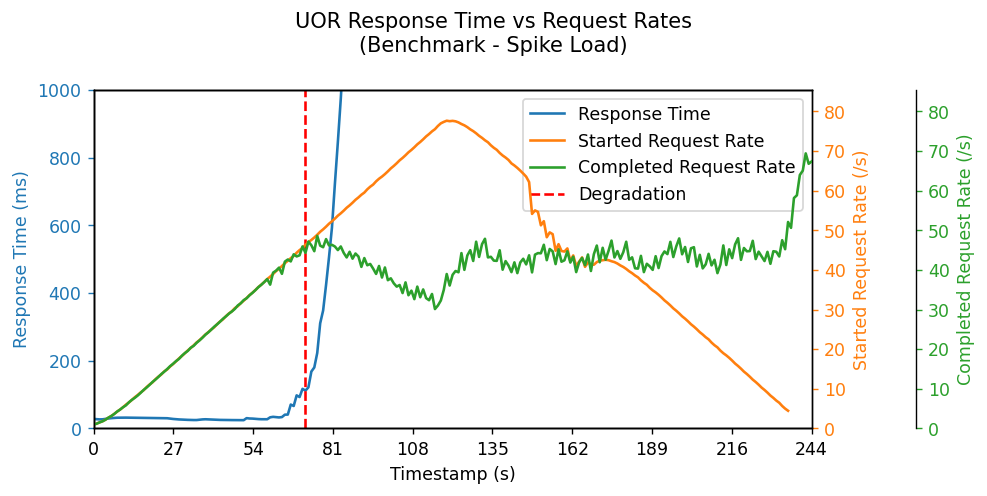
\includegraphics[width=0.8\textwidth]{figures/uor-benchmark-spike.png}
    \caption{UOR response time vs. request rate graph - spike load benchmark}
    \label{figure:uor-benchmark-spike}
\end{figure}

\begin{figure}[h]
    \centering
    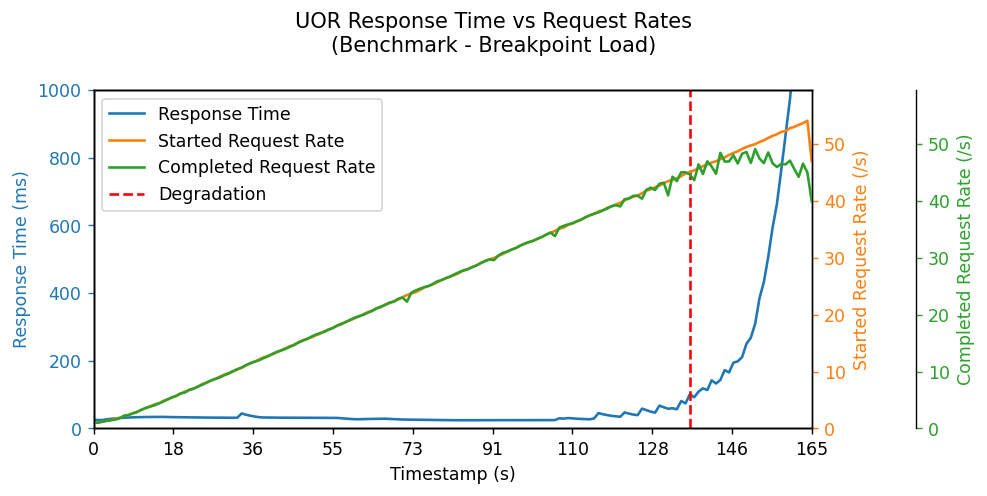
\includegraphics[width=0.8\textwidth]{figures/uor-benchmark-breakpoint.png}
    \caption{UOR response time vs. request rate graph - breakpoint load benchmark}
    \label{figure:uor-benchmark-breakpoint}
\end{figure}

As seen in Fig. \ref{figure:uor-benchmark-average}, a local deployment of the Ahuora Digital Platform is able to sustain a request completion rate of 15 requests per second (from the average load profile), matching the number of requests received per second. The response time is also relatively consistent, ranging between 27 and 30 milliseconds on average. When the stress load profile is applied (30 requests per second), the average response time decreases to \textasciitilde25 milliseconds (Fig. \ref{figure:uor-benchmark-stress}). The system also continues to process requests at the request rate, with only slightly more inconsistency than the average load test. The response time decrease seen with the stress profile compared with the average profile could be the result of the API making more use of a cache layer within the system.

Both response time and request rate degradation can be observed in the local spike test (Fig. \ref{figure:uor-benchmark-spike}). After reaching \textasciitilde40 requests per second, the response time rapidly increases, and the request completion rate starts to diverge from the request start rate. At 45 requests per second (RPS), the response time average increases past 100 milliseconds, and reaches tens of thousands of milliseconds as the request rate continues to increase. During the test, the request start rate is also seen degrading (between 135 and 189 seconds). This is because of the virtual user limit of 2000 set on the k6 test client, which was configured to prevent system resource starvation by the test client. The response time does not appear to recover towards the end of the test.

The breakpoint test (Fig. \ref{figure:uor-benchmark-breakpoint}) also identifies this 44 RPS threshold beyond which the average response time exceeds 100 milliseconds, and the request completion rate also diverges.

% Update these ^^ thresholds based on average values

\subsection{Replica count}


\subsection{Resource allocation and utilisation}


% \subsection{Minimum replicas}
% \subsubsection{Average load}
% \subsubsection{Stress load}
% \subsubsection{Spike load}
% \subsubsection{Breakpoint load}

\section{Flowsheet solving (FS) experiment results}

\subsection{Benchmarks}


\subsection{Replica count}


\subsection{Resource allocation and utilisation}


% \subsection{Minimum replicas}
% \subsubsection{Average load}
% \subsubsection{Stress load}
% \subsubsection{Spike load}
% \subsubsection{Breakpoint load}

\section{Impacts}
Efficiency, accuracy, feasibility (examples of demonstrable impacts).
\section{Threats to validity}